\chapter{Análises classificatórias}

Por mais que houve o estudo realizado na área de reconhecimento de padrões em \textit{machine learning}, após o recebimento da base foi notado que a base era composta principalmente por instâncias rotuladas, ou seja, as classes eram conhecidas e possíveis de categorização. Além disso, já que a base não está afirmando quais alunos irão evadir, apenas mostrando respostas possíveis de estudantes a um questionário, é mais interessante de um ponto de vista científico afirmar quais variáveis possuem o maior peso de predição de influência dentro do questionário. Sendo assim, foi concluído que a melhor estratégia adotada para o trabalho foi não a de reconhecer padrões, mas sim a de aplicação de técnicas de classificação em \textit{machine learning}, sem alteração nos algoritmos que serão utilizados para análise.

Para fazer a aplicação dos métodos na base, alguns cuidados foram necessários para que os modelos não tivessem problemas em suas análises e treinamento.

O primeiro passo foi retratar os dados de valores reais para valores inteiros. Isso acontece porque, como estamos lidando com um problema de classificação, cada fração seria considerada uma classe diferente. Ou seja, valores como ``3.0'' e ``3.333333'' são considerados duas classes diferentes. Para que fosse melhor identificado a classe que um aluno poderia estar, foi arredondado todos os valores de ponto flutuante, arredondando os valores para cima caso tivessem sua primeira casa após a vírgula 5 em diante (ou seja, valores como 2.5 e 2.6666667 foram considerados 3.0, enquanto 2.3333333 foi considerado 2).

Além disso, como é possível verificar pelos histogramas das Figuras \ref{fig:histograma-dimensoes} e \ref{fig:histograma-fatores}, havia um severo desbalanceamento da base em todas as variáveis, tanto nas categorias de dimensão quanto na de fatores. Para cada variável, havia grande número de respostas distribuídas entre os valores 1 a 3, e poucas respostas classificadas entre 5 a 7. Isso significa que foi necessário realizar um balanceamento da base, evitando um desempenho enviesado em relação a uma das classes. Apenas durante o treinamento dos modelos para cada dimensão e cada fator, foi escolhida a classe com o maior número de respostas, e todas as outras classes foram redistribuídas.

\begin{figure}[htp!]
    \centering
    \caption{Histograma Dimensões}
    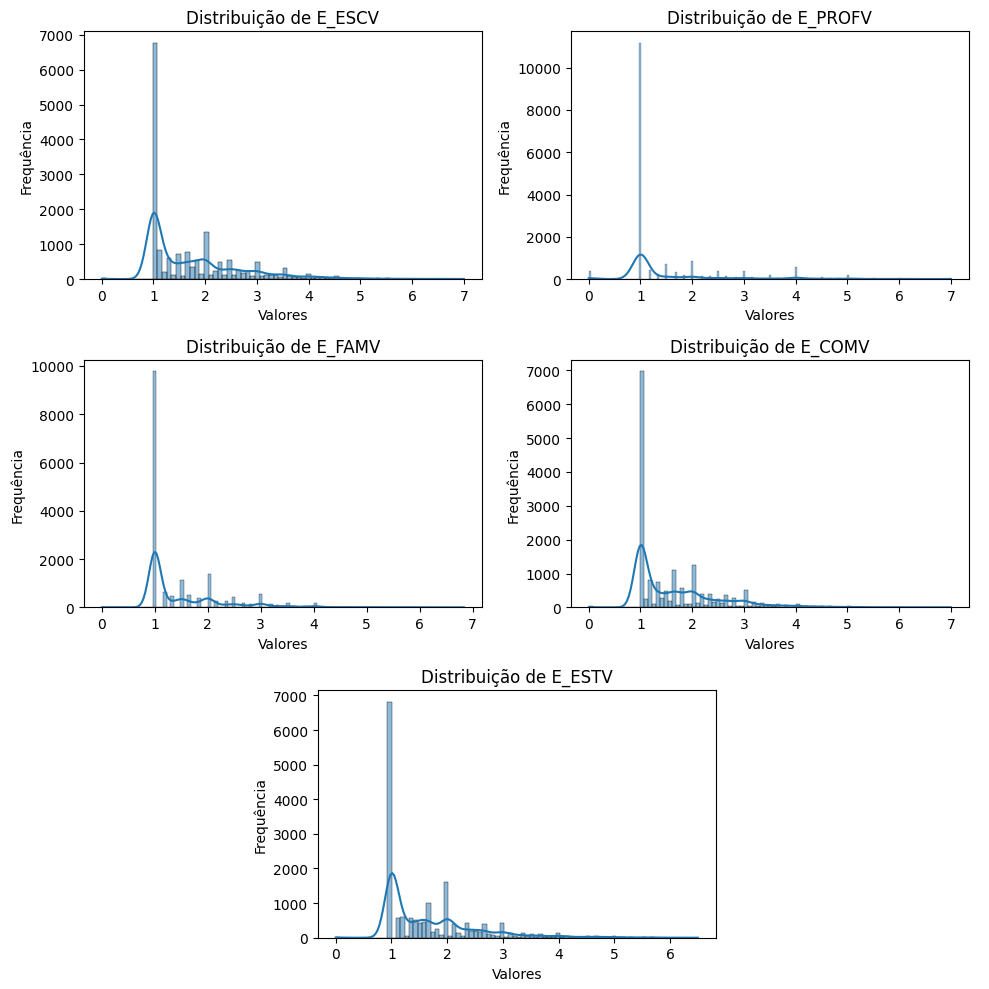
\includegraphics[width=0.75\textwidth]{Textuais/Imagens/Gráficos/histograma_dimensoes.png}
    \label{fig:histograma-dimensoes}
    \fonte{\me{2023}}
\end{figure}

\begin{figure}[htp!]
    \centering
    \caption{Histograma Fatores}
    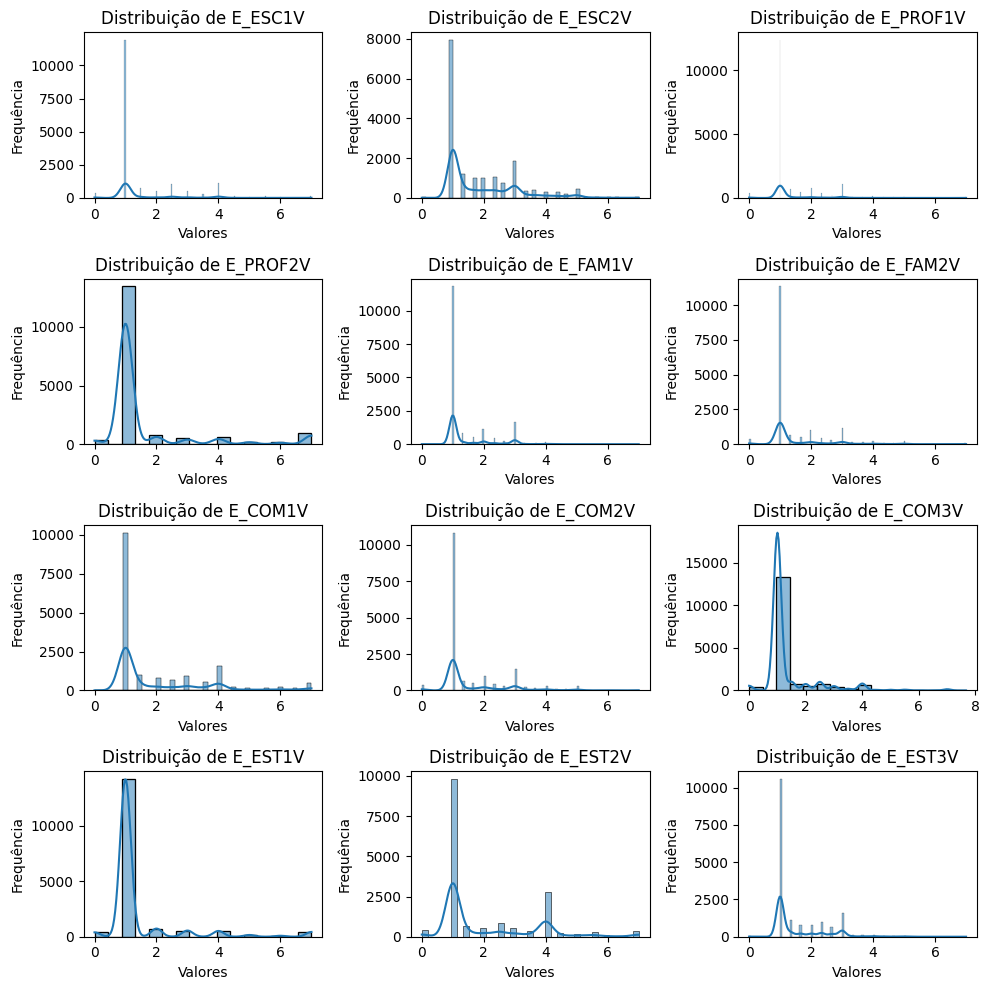
\includegraphics[width=0.8\textwidth]{Textuais/Imagens/Gráficos/histograma_fatores.png}
    \label{fig:histograma-fatores}
    \fonte{\me{2023}}
\end{figure}

Também é importante informar que durante os testes, não foram divididos de forma fixa conjunto de dados para treinamento, teste e validação, e eles eram distintos entre si. A cada iteração do código, 20\% da base era aleatoriamente escolhida para tratar como teste, querendo evitar desempenhos superestimados, pois caso não fosse tomado esse cuidado, os modelos já teriam visto os dados de teste durante o treinamento.

É relevante informar que para além das métricas escolhidas para avaliação dos modelos como consta na seção \ref{subsec:tecnicas}, também foram feitas a visualização das matrizes de confusão para melhor compreensão acerca da \textit{performance} dos modelos escolhidos. Todas as matrizes de confusão encontram-se nos Apêndices \ref{ap1}, \ref{ap2}, \ref{ap3}, \ref{ap4} e \ref{ap5} deste trabalho.

Por fim, os algoritmos foram todos treinados utilizando a linguagem de programação Python 3.10, com o auxílio da biblioteca \textit{sklearn}. Foram utilizados os seguintes modelos para treinamento dentro da biblioteca: DecisionTreeClassifier, RandomForestClassifier, AdaBoostClassifier, CategoricalNB e KNeighborsClassifier. Os algoritmos foram testados em uma máquina que continha as seguintes especificações: \textit{OS: Windows 10 19045.3448 x86\_64;
RAM: 24 GB;
CPU: Intel Core(TM) i5-7400 CPU @ 3.00GHz;
GPU: RTX 3060 12GB}.

A seguir, são apresentados os resultados dos algoritmos escolhidos após sua aplicação no banco de dados, destacando as variáveis que obtiveram os melhores resultados classificatórios.

\section{Decision Tree}

A análise das Tabelas \ref{tab:dimensoes_decision_tree_classifier} e \ref{tab:fatores_decision_tree} revela algumas informações importantes sobre o desempenho do modelo de Decision Tree nas diferentes dimensões testadas. Inicialmente, é perceptível que os valores de acurácia para todas as variáveis são relativamente altos, variando de aproximadamente 74\% a 99\%, indicando, em geral, uma boa capacidade do modelo em prever corretamente as classes.

\begin{table}[ht]
    \centering
    \caption{Dimensões sendo testadas no modelo de Decision Tree}
    \resizebox{0.8\textwidth}{!}{%
    \begin{tabular}{|c|c|c|c|c|}
    \hline
    \textbf{Variável} & \textbf{Acurácia} & \textbf{Precisão} & \textbf{Recall Score} & \textbf{F1 Score} \\ \hline
    \textbf{E\_ESCV}  & 0.751673360 & 0.739981653 & 0.751673360 & 0.741630082 \\ \hline
    \textbf{E\_PROFV} & 0.783035930 & 0.786358820 & 0.783035930 & 0.777129550 \\ \hline
    \textbf{E\_FAMV}  & 0.830982219 & 0.831129806 & 0.830982219 & 0.827472004 \\ \hline
    \textbf{E\_COMV}  & 0.774183466 & 0.769368781 & 0.774183466 & 0.767111565 \\ \hline
    \textbf{E\_ESTV}  & 0.741793911 & 0.732561420 & 0.741793911 & 0.732551048 \\ \hline
    \end{tabular}%
    }
    \label{tab:dimensoes_decision_tree_classifier}
    \fonte{\me{2023}}
\end{table}

\begin{table}[ht]
    \centering
    \caption{Fatores sendo testados no modelo Decision Tree}
    \resizebox{0.8\textwidth}{!}{%
    \begin{tabular}{|c|c|c|c|c|}
        \hline
        \textbf{Variável} & \textbf{Acurácia} & \textbf{Precisão} & \textbf{Recall Score} & \textbf{F1 Score} \\ \hline
        \textbf{E\_ESC1V}  & 0.973298932 & 0.974228894 & 0.973298932 & 0.972954891 \\ \hline
        \textbf{E\_ESC2V}  & 0.957975316 & 0.958817154 & 0.957975316 & 0.957990201 \\ \hline
        \textbf{E\_PROF1V} & 0.985004378 & 0.985474842 & 0.985004378 & 0.984873283 \\ \hline
        \textbf{E\_PROF2V} & 0.995594947 & 0.995617592 & 0.995594947 & 0.995594299 \\ \hline
        \textbf{E\_FAM1V}  & 0.981763607 & 0.982526522 & 0.981763607 & 0.981566092 \\ \hline
        \textbf{E\_FAM2V}  & 0.988539873 & 0.988990114 & 0.988539873 & 0.988512460 \\ \hline
        \textbf{E\_COM1V}  & 0.957073377 & 0.958085738 & 0.957073377 & 0.956205580 \\ \hline
        \textbf{E\_COM2V}  & 0.977282629 & 0.978631022 & 0.977282629 & 0.976942412 \\ \hline
        \textbf{E\_COM3V}  & 0.988506982 & 0.989023192 & 0.988506982 & 0.988421136 \\ \hline
        \textbf{E\_EST1V}  & 0.987947572 & 0.988248921 & 0.987947572 & 0.987787534 \\ \hline
        \textbf{E\_EST2V}  & 0.973289665 & 0.974189465 & 0.973289665 & 0.973112790 \\ \hline
        \textbf{E\_EST3V}  & 0.986756179 & 0.987237780 & 0.986756179 & 0.986687563 \\ \hline
    \end{tabular}%
    }
    \fonte{\me{2023}}
    \label{tab:fatores_decision_tree}
\end{table}

Ao observar as métricas de precisão, recall e F1 Score, nota-se uma consistência nos resultados para cada variável. No geral, as métricas de precisão e recall são bastante equilibradas, indicando que o modelo consegue manter um bom equilíbrio entre a identificação correta das instâncias positivas e a minimização de falsos positivos.

Entretanto, ao analisar mais profundamente, percebe-se que o fator \textbf{E\_ESC1V} (Condições Materiais da Escola) se destaca com valores extremamente altos em todas as métricas, com acurácia, precisão, recall e F1 Score superiores a 97\%. Isso sugere que o modelo possui um desempenho excepcional ao lidar com essa variável específica, indicando possivelmente uma característica única ou padrão distinto nessa dimensão.

Por outro lado, a dimensão \textbf{E\_ESTV} (Estudante-Estudante) apresenta valores ligeiramente inferiores em comparação com as outras variáveis, especialmente em termos de acurácia e F1 Score. Isso pode indicar que essa dimensão é mais desafiadora para o modelo, seja devido à complexidade dos padrões presentes nos dados ou a uma menor representatividade das características distintivas.

Comparando as métricas, nota-se que, considerando a acurácia geral, o fator \textbf{E\_ESC1V} se destaca. No entanto, as dimensões \textbf{E\_PROFV} (Estudante-Profissionais da
Escola)  ou \textbf{E\_FAMV} (Estudante-Família) também se destacam por possuírem equilíbrio entre precisão e recall. Por outro lado, a pior variável para predição, ou seja, que apresentou os piores valores nas métricas, é a dimensão \textbf{E\_ESTV} (Estudante-Estudante).


%%%%%%%%%%%%%%%%%%%%%%%%%%%

\section{Random Forest}

Ao analisar as Tabelas \ref{tab:dimensoes_random_forest_classifier} e \ref{tab:fatores_random_forest_classifier}, algumas observações são notáveis. Na tabela referente às dimensões, as variáveis \textbf{E\_ESCV} (Estudante-Escola) \textbf{E\_FAMV} (Estudante-Família) se destacam com os maiores valores em todas as métricas, indicando um bom desempenho global do modelo nas duas dimensões.

\begin{table}[ht]
    \centering
    \caption{Dimensões sendo testadas no modelo Random Forest}
    \resizebox{0.8\textwidth}{!}{%
    \begin{tabular}{|c|c|c|c|c|}
    \hline
    \textbf{Variável} & \textbf{Acurácia} & \textbf{Precisão} & \textbf{Recall Score} & \textbf{F1 Score} \\ \hline
    \textbf{E\_ESCV}  & 0.848055295	& 0.842921845 & 0.848055295 & 0.843924479 \\ \hline
    \textbf{E\_PROFV} & 0.786592718 & 0.790278008 & 0.786592718 & 0.781311994 \\ \hline
    \textbf{E\_FAMV}  & 0.833147431 & 0.831530566 & 0.833147431 & 0.829228533 \\ \hline
    \textbf{E\_COMV}  & 0.778324738 & 0.770605436 & 0.778324738 & 0.771282145 \\ \hline
    \textbf{E\_ESTV}  & 0.744445460 & 0.734167526 & 0.744445460 & 0.735079615 \\ \hline
    \end{tabular}%
    }
    \fonte{\me{2023}}
    \label{tab:dimensoes_random_forest_classifier}
\end{table}

\begin{table}[ht]
    \centering
    \caption{Fatores sendo testados no modelo Random Forest}
    \resizebox{0.8\textwidth}{!}{%
    \begin{tabular}{|c|c|c|c|c|}
        \hline
        \textbf{Variável} & \textbf{Acurácia} & \textbf{Precisão} & \textbf{Recall Score} & \textbf{F1 Score} \\ \hline
        \textbf{E\_ESC1V}  & 0.979659186 & 0.980308426 & 0.979659186 & 0.979535759 \\ \hline
        \textbf{E\_ESC2V}  & 0.964458678 & 0.964734405 & 0.964458678 & 0.964430198 \\ \hline
        \textbf{E\_PROF1V} & 0.988178634 & 0.988461239 & 0.988178634 & 0.988120343 \\ \hline
        \textbf{E\_PROF2V} & 0.996337968 & 0.996351606 & 0.996337968 & 0.996338277 \\ \hline
        \textbf{E\_FAM1V}  & 0.982499858 & 0.983288480 & 0.982499858 & 0.982314134 \\ \hline
        \textbf{E\_FAM2V}  & 0.990855650 & 0.991095707 & 0.990855650 & 0.990836153 \\ \hline
        \textbf{E\_COM1V}  & 0.968210333 & 0.968547724 & 0.968210333 & 0.967829172 \\ \hline
        \textbf{E\_COM2V}  & 0.982635215 & 0.983218686 & 0.982635215 & 0.982435642 \\ \hline
        \textbf{E\_COM3V}  & 0.992910849 & 0.993159647 & 0.992910849 & 0.992893850 \\ \hline
        \textbf{E\_EST1V}  & 0.996836238 & 0.996854884 & 0.996836238 & 0.996829868 \\ \hline
        \textbf{E\_EST2V}  & 0.981295488 & 0.981635502 & 0.981295488 & 0.981176100 \\ \hline
        \textbf{E\_EST3V}  & 0.987244431 & 0.987795643 & 0.987244431 & 0.987156619 \\ \hline
    \end{tabular}%
    }
    \fonte{\me{2023}}
    \label{tab:fatores_random_forest_classifier}
\end{table}

No entanto, ao examinar os fatores, é evidente que a maioria das variáveis atingiu altos níveis de desempenho, com valores de acurácia, precisão, recall e F1 score consistentemente elevados. Destacam-se particularmente as variáveis \textbf{E\_EST1V} (Significados da Escolarização/Engajamento) e \textbf{E\_COM3V} (Distanciamento escola – comunidade), que apresentam desempenho praticamente impecável em todas as métricas avaliadas.

% Ao considerar a melhor dimensão para predição, destaca-se \textbf{E\_FAMV} devido aos seus valores mais altos. Por outro lado, ao observar a precisão e o recall, as variáveis em \textbf{Fatores} se destacam, especialmente \textbf{E\_EST1V} e \textbf{E\_COM3V}.



%%%%%%%%%%%%%%%%%%%%%%%%%%%

\section{Adaboost}

Ao analisar as Tabelas \ref{tab:dimensoes_adaboost_classifier} e \ref{tab:fatores_adaboost_classifier} fica evidente que as métricas de desempenho do modelo Adaboost variam significativamente entre as diferentes variáveis testadas.

\begin{table}[ht]
    \centering
    \caption{Dimensões sendo testadas no modelo Adaboost}
    \resizebox{0.8\textwidth}{!}{%
    \begin{tabular}{|c|c|c|c|c|}
    \hline
    \textbf{Variável} & \textbf{Acurácia} & \textbf{Precisão} & \textbf{Recall Score} & \textbf{F1 Score} \\ \hline
    \textbf{E\_ESCV}  & 0.310408300 & 0.283796729 & 0.310408300 & 0.290538426 \\ \hline
    \textbf{E\_PROFV} & 0.271883289 & 0.264811380 & 0.271883289 & 0.263795898 \\ \hline
    \textbf{E\_FAMV}  & 0.300177154 & 0.516699197 & 0.300177154 & 0.218699253 \\ \hline
    \textbf{E\_COMV}  & 0.302390999 & 0.289724284 & 0.302390999 & 0.284777157 \\ \hline
    \textbf{E\_ESTV}  & 0.295144921 & 0.281181766 & 0.295144921 & 0.272988844 \\ \hline
    \end{tabular}%
    }
    \fonte{\me{2023}}
    \label{tab:dimensoes_adaboost_classifier}
\end{table}

\begin{table}[ht]
    \centering
    \caption{Fatores sendo testados no modelo Adaboost}
    \resizebox{0.8\textwidth}{!}{%
    \begin{tabular}{|c|c|c|c|c|}
        \hline
        \textbf{Variável} & \textbf{Acurácia} & \textbf{Precisão} & \textbf{Recall Score} & \textbf{F1 Score} \\ \hline
        \textbf{E\_ESC1V}  & 0.358454338 & 0.342833509 & 0.358454338 & 0.320662206 \\ \hline
        \textbf{E\_ESC2V}  & 0.362599594 & 0.408169540 & 0.362599594 & 0.330145255 \\ \hline
        \textbf{E\_PROF1V} & 0.439306042 & 0.444431554 & 0.439306042 & 0.430396321 \\ \hline
        \textbf{E\_PROF2V} & 0.371563528 & 0.429579049 & 0.371563528 & 0.339875124 \\ \hline
        \textbf{E\_FAM1V}  & 0.517981537 & 0.805497664 & 0.517981537 & 0.415171182 \\ \hline
        \textbf{E\_FAM2V}  & 0.281396592 & 0.636934146 & 0.281396592 & 0.155494301 \\ \hline
        \textbf{E\_COM1V}  & 0.416367097 & 0.409562625 & 0.416367097 & 0.397870672 \\ \hline
        \textbf{E\_COM2V}  & 0.333478559 & 0.368666728 & 0.333478559 & 0.319560681 \\ \hline
        \textbf{E\_COM3V}  & 0.449838883 & 0.520024864 & 0.449838883 & 0.454163910 \\ \hline
        \textbf{E\_EST1V}  & 0.465022849 & 0.458395635 & 0.465022849 & 0.454569975 \\ \hline
        \textbf{E\_EST2V}  & 0.381586608 & 0.425480643 & 0.381586608 & 0.382408663 \\ \hline
        \textbf{E\_EST3V}  & 0.318156851 & 0.338854607 & 0.318156851 & 0.273703286 \\ \hline
    \end{tabular}%
    }
    \fonte{\me{2023}}
    \label{tab:fatores_adaboost_classifier}
\end{table}

Observando a Tabela \ref{tab:dimensoes_adaboost_classifier}, é notável que as variáveis relacionadas à educação (\textbf{E\_ESCV} (Estudante-Escola), \textbf{E\_PROFV} (Estudante-Profissionais da Escola), \textbf{E\_FAMV} (Estudante-Família), \textbf{E\_COMV} (Estudante-Escola), E\_ESTV (Estudante-Estudante)) têm desempenhos relativamente baixos em todas as métricas. A variável \textbf{E\_FAMV}, em particular, destaca-se pela sua baixa precisão e F1 Score, indicando que o modelo tem dificuldade em fazer previsões precisas e equilibradas para essa dimensão.

Já com relação à Tabela \ref{tab:fatores_adaboost_classifier}, é possível observar uma variabilidade mais ampla nos resultados. Alguns fatores, como \textbf{E\_FAM1V} (Suporte Familiar), \textbf{E\_COM3V} (Distanciamento Escola-Comunidade) e \textbf{E\_EST1V} (Significados da Escolarização/Engajamento), mostram desempenhos mais promissores em comparação com outras, como é o caso do fator \textbf{E\_FAM1V} que possui uma acurácia relativamente alta.


%%%%%%%%%%%%%%%%%%%%%%%%%%%

\section{Naive Bayes Categórico}

Ao analisar as Tabelas \ref{tab:dim_naive_bayes_classifier} e \ref{tab:fatores_naive_bayes_classifier}, chama a atenção a grande variabilidade nos valores de acurácia, precisão, recall e F1 Score entre as diferentes variáveis testadas.

\begin{table}[ht]
\caption{Dimensões sendo testadas no modelo Naive Bayes Categórico}
    \centering
    \resizebox{0.8\textwidth}{!}{%
    \begin{tabular}{|c|c|c|c|c|}
    \hline
    \textbf{Variável} & \textbf{Acurácia} & \textbf{Precisão} & \textbf{Recall Score} & \textbf{F1 Score} \\ \hline
    \textbf{E\_ESCV}  & 0.457914993 & 0.434943418 & 0.457914993 & 0.428372704 \\ \hline
    \textbf{E\_PROFV} & 0.411020014 & 0.407000983 & 0.411020014 & 0.400572047 \\ \hline
    \textbf{E\_FAMV}  & 0.618463355 & 0.598444859 & 0.618463355 & 0.601411496 \\ \hline
    \textbf{E\_COMV}  & 0.494374121 & 0.467487650 & 0.494374121 & 0.472578934 \\ \hline
    \textbf{E\_ESTV}  & 0.433299808 & 0.414196732 & 0.433299808 & 0.406825414 \\ \hline
    \end{tabular}%
    }
    \fonte{\me{2023}}
    \label{tab:dim_naive_bayes_classifier}
\end{table}

\begin{table}[ht]
\caption{Fatores sendo testados no modelo Naive Bayes Categórico}
    \centering
    \resizebox{0.8\textwidth}{!}{%
    \begin{tabular}{|c|c|c|c|c|}
    \hline
    \textbf{Variável} & \textbf{Acurácia} & \textbf{Precisão} & \textbf{Recall Score} & \textbf{F1 Score} \\ \hline
    \textbf{E\_ESC1V}  & 0.561202448 & 0.555537424 & 0.561202448 & 0.556714967 \\ \hline
    \textbf{E\_ESC2V}  & 0.563427589 & 0.555158840 & 0.563427589 & 0.558275101 \\ \hline
    \textbf{E\_PROF1V} & 0.637259194 & 0.638644712 & 0.637259194 & 0.635457652 \\ \hline
    \textbf{E\_PROF2V} & 0.616813502 & 0.610137577 & 0.616813502 & 0.611076953 \\ \hline
    \textbf{E\_FAM1V}  & 0.750127428 & 0.744078395 & 0.750127428 & 0.745922676 \\ \hline
    \textbf{E\_FAM2V}  & 0.640163886 & 0.636322205 & 0.640163886 & 0.636805646 \\ \hline
    \textbf{E\_COM1V}  & 0.529216889 & 0.528650634 & 0.529216889 & 0.522478593 \\ \hline
    \textbf{E\_COM2V}  & 0.519138607 & 0.513238162 & 0.519138607 & 0.513408647 \\ \hline
    \textbf{E\_COM3V}  & 0.629699248 & 0.636854980 & 0.629699248 & 0.630850677 \\ \hline
    \textbf{E\_EST1V}  & 0.567317833 & 0.568723238 & 0.567317833 & 0.563402589 \\ \hline
    \textbf{E\_EST2V}  & 0.482168850 & 0.482410913 & 0.482168850 & 0.474973736 \\ \hline
    \textbf{E\_EST3V}  & 0.758010375 & 0.761468350 & 0.758010375 & 0.758019485 \\ \hline
    \end{tabular}%
    }
    \fonte{\me{2023}}
    \label{tab:fatores_naive_bayes_classifier}
\end{table}

Na Tabela \ref{tab:dim_naive_bayes_classifier} destaca-se a variável \textbf{E\_FAMV} (Estudante-Família) por apresentar os maiores valores em todas as métricas, indicando um desempenho geral mais consistente. Isso sugere que esta dimensão possui uma capacidade significativa de predição para o modelo Naive Bayes Categórico. Por outro lado, a variável \textbf{E\_PROFV} (Estudante-Profissionais da Escola) mostra valores mais baixos em todas as métricas, demonstrando sua baixa eficácia.

Na Tabela \ref{tab:fatores_naive_bayes_classifier}, observa-se que as variáveis relacionadas à interação do estudante dentro da escola (\textbf{E\_ESC1V}, \textbf{E\_ESC2V}, \textbf{E\_PROF1V}, \textbf{E\_PROF2V}, \textbf{E\_EST1V}, \textbf{E\_EST2V}, \textbf{E\_EST3V}) e com sua família (\textbf{E\_FAM1V}, \textbf{E\_FAM2V}) apresentam resultados gerais mais elevados em comparação com as variáveis relacionadas à relação do estudante com a comunidade (\textbf{E\_COM1V}, \textbf{E\_COM2V}, \textbf{E\_COM3V}).





%%%%%%%%%%%%%%%%%%%%%%%%%%%

\section{K Vizinhos Próximos}

Olhando para a Tabela \ref{tab:dimensoes_knn_classifier}, é possível notar que todas as variáveis têm valores relativamente próximos para cada métrica, indicando consistência no desempenho do modelo. No entanto, a variável \textbf{E\_FAMV} (Estudante-Família) destaca-se por apresentar valores ligeiramente mais altos em todas as métricas, sugerindo que essa dimensão pode ser a mais promissora para a predição com base nos resultados fornecidos.

Já ao examinar a Tabela \ref{tab:fatores_knn_classifier}, que parece representar diferentes fatores testados no mesmo modelo, observa-se uma variação mais significativa nas métricas de desempenho, sendo que a variável \textbf{E\_FAM1V} (Suporte Familiar) se destaca como a que possui os valores mais elevados em todas as métricas.


\begin{table}[ht]
    \centering
    \caption{Dimensões sendo testadas no modelo K Vizinhos Próximos}
    \resizebox{0.8\textwidth}{!}{%
    \begin{tabular}{|c|c|c|c|c|}
        \hline
        \textbf{Variável} & \textbf{Acurácia} & \textbf{Precisão} & \textbf{Recall Score} & \textbf{F1 Score} \\ \hline
        \textbf{E\_ESCV}  & 0.711596386 & 0.700557792 & 0.711596386 & 0.704636645 \\ \hline
        \textbf{E\_PROFV} & 0.738606221 & 0.700557792 & 0.738606221 & 0.734757179 \\ \hline
        \textbf{E\_FAMV}  & 0.805524572 & 0.700557792 & 0.805524572 & 0.802252778 \\ \hline
        \textbf{E\_COMV}  & 0.731598687 & 0.700557792 & 0.731598687 & 0.725306201 \\ \hline
        \textbf{E\_ESTV}  & 0.708512389 & 0.698463926 & 0.708512389 & 0.701349474 \\ \hline
    \end{tabular}%
    }
    \fonte{\me{2023}}
    \label{tab:dimensoes_knn_classifier}
\end{table}

\begin{table}[ht]
    \centering
    \caption{Fatores sendo testados no modelo K Vizinhos Próximos}
    \resizebox{0.8\textwidth}{!}{%
    \begin{tabular}{|c|c|c|c|c|}
        \hline
        \textbf{Variável} & \textbf{Acurácia} & \textbf{Precisão} & \textbf{Recall Score} & \textbf{F1 Score} \\ \hline
        \textbf{E\_ESC1V}  & 0.742289692 & 0.740910883 & 0.742289692 & 0.737724470 \\ \hline
        \textbf{E\_ESC2V}  & 0.666536479 & 0.660486864 & 0.666536479 & 0.660315920 \\ \hline
        \textbf{E\_PROF1V} & 0.785573555 & 0.790021952 & 0.785573555 & 0.782115192 \\ \hline
        \textbf{E\_PROF2V} & 0.749655026 & 0.757937584 & 0.749655026 & 0.747544018 \\ \hline
        \textbf{E\_FAM1V}  & 0.841989013 & 0.839724686 & 0.841989013 & 0.839231689 \\ \hline
        \textbf{E\_FAM2V}  & 0.734576332 & 0.736068762 & 0.734576332 & 0.731472431 \\ \hline
        \textbf{E\_COM1V}  & 0.652075844 & 0.652540182 & 0.652075844 & 0.649568168 \\ \hline
        \textbf{E\_COM2V}  & 0.716686376 & 0.716540340 & 0.716686376 & 0.712667529 \\ \hline
        \textbf{E\_COM3V}  & 0.804296455 & 0.805046405 & 0.804296455 & 0.800538307 \\ \hline
        \textbf{E\_EST1V}  & 0.774569377 & 0.782217841 & 0.774569377 & 0.772245486 \\ \hline
        \textbf{E\_EST2V}  & 0.679184862 & 0.674932518 & 0.679184862 & 0.672756158 \\ \hline
        \textbf{E\_EST3V}  & 0.802807446 & 0.801495596 & 0.802807446 & 0.800699248 \\ \hline
    \end{tabular}%
    }
    \fonte{\me{2023}}
    \label{tab:fatores_knn_classifier}
\end{table}

A variável \textbf{E\_COM2V} (Acessibilidade e frequência escolar) na segunda tabela parece ter um desempenho relativamente inferior em comparação com outras variáveis, destacando-se como a menos promissora para a predição com base nos valores fornecidos. Portanto, as dimensões \textbf{E\_FAMV} (Estudante-Família) na primeira tabela e \textbf{E\_FAM1V} (Suporte Familiar) na segunda tabela são as mais promissoras para predição, enquanto \textbf{E\_COM2V} pode ser considerada menos favorável.

Concluindo a análise de todos os algoritmos e seus resultados, agora realiza-se uma análise comparativa entre cada um.



\subsection{Análise comparativa}



A análise comparativa dos algoritmos de \textit{machine learning} utilizados neste estudo revela o desempenho de cada um no contexto da classificação de variáveis educacionais. Ao examinar os principais aspectos de cada modelo para determinar qual foi o mais eficaz:

\begin{itemize}
    \item Decision Tree: Este modelo mostrou alta capacidade de prever corretamente as classes, com acurácias variando de aproximadamente 74\% a 99\% em diferentes variáveis. A variável \textbf{E\_ESC1V} (Condições Materiais da Escola) se destacou com valores excepcionalmente altos em todas as métricas, indicando um desempenho particularmente forte nesta dimensão.

    \item Random Forest: Demonstrou ser eficiente em várias dimensões, com destaque para \textbf{E\_FAMV} (Estudante Família) nas dimensões e \textbf{E\_EST1V} (Condições Materiais da Escola) e \textbf{E\_COM3V} (Distanciamento escola – comunidade) nos fatores, todas apresentando altos valores de desempenho. Este modelo parece ter uma capacidade geral superior em lidar com uma variedade maior de dimensões e fatores.

    \item AdaBoost: Apresentou uma variabilidade considerável nos resultados, com algumas variáveis mostrando desempenhos promissores, como \textbf{E\_FAM1V} (Suporte Familiar) e \textbf{E\_COM3V} (Distanciamento escola – comunidade), enquanto outras apresentaram desafios significativos, especialmente nas dimensões relacionadas à educação.

    \item Naive Bayes Categórico: Este modelo teve um desempenho variado, com \textbf{E\_FAMV} (Estudante-Família) destacando-se nas dimensões e várias variáveis relacionadas à escola mostrando resultados mais elevados entre os fatores. No entanto, houve uma variação notável entre as diferentes variáveis testadas.

    \item K Vizinhos Próximos (KNN): Apresentou consistência em seu desempenho, com \textbf{E\_FAMV} (Estudante-Família) e \textbf{E\_FAM1V} (Suporte Familiar) emergindo como as dimensões mais promissoras para predição.
\end{itemize}



Considerando todos os aspectos, o Random Forest mostra-se o algoritmo mais robusto e versátil para este conjunto de dados. Ele não apenas demonstrou alta eficácia em uma ampla gama de variáveis, mas também mostrou um bom equilíbrio entre precisão e recall, indicando sua capacidade de lidar com diferentes tipos de dados de maneira eficiente. Além disso, a natureza do Random Forest, que agrega as decisões de várias árvores de decisão, contribui para sua robustez e capacidade de lidar com complexidades e nuances nos dados educacionais. Portanto, o Random Forest é recomendado como o algoritmo mais adequado para este estudo, com base em sua performance geral e capacidade de lidar com uma variedade de variáveis educacionais de forma eficaz.

Portanto, é chego à conclusão que as variáveis que melhor performam, independente do algoritmo, são  E\_FAM1V (Suporte Familiar) e E\_COM3V (Distanciamento escola – comunidade) para os fatores, e E\_FAMV (Estudante-Família) para as dimensões, sendo estas os fatores de risco de evasão que possuem mais proeminência na base.

% O Random Forest se destaca no universo dos algoritmos de \textit{machine learning}, particularmente no tratamento de dados complexos como aqueles encontrados no setor educacional. Sua eficiência advém de uma abordagem de aprendizado de ensemble, onde várias árvores de decisão são combinadas para formar um modelo mais forte e mais confiável. Esta estratégia é fundamental para diminuir o risco de overfitting, um desafio comum em modelos mais simples.

% A capacidade do Random Forest de reduzir a variância sem aumentar o viés é uma de suas maiores forças. Isto significa que o modelo é capaz de generalizar de forma mais eficaz para novos dados, mantendo uma performance consistente tanto em dados de treino quanto em dados de teste. Esta característica é de grande valor no contexto educacional, onde a diversidade de dados e a necessidade de generalização são fatores críticos.

% Além disso, a flexibilidade do Random Forest em lidar com diferentes tipos de dados é uma vantagem incontestável. Ele pode processar dados categóricos e contínuos e se adapta bem a grandes volumes de dados e a um vasto número de variáveis de entrada, que são características comuns em análises no campo da educação.

% Outro ponto forte do Random Forest é sua habilidade em determinar a importância de cada variável no processo de decisão. Essa capacidade é essencial em estudos educacionais, pois ajuda a identificar os fatores mais impactantes em questões como a evasão escolar. Compreender quais variáveis têm maior influência pode ser o diferencial para implementar políticas educacionais mais efetivas e intervenções focadas.

% O Random Forest também mostra resiliência frente a desafios como dados faltantes e desbalanceamento de classes, problemas frequentemente encontrados em dados educacionais. Ele pode tratar valores faltantes utilizando estratégias como a média ou a moda, e seu método de bagging ajuda a equilibrar o impacto de classes desiguais.

% Portanto, devido à sua versatilidade, robustez e precisão, o Random Forest é uma escolha excelente para a análise de dados educacionais. Ele integra com sucesso uma ampla gama de informações, lidando eficientemente com os desafios apresentados pelos dados educacionais. É esta combinação de características que faz dele o algoritmo mais recomendado para o conjunto de dados analisados no presente estudo.